\documentclass[a4paper]{article}
\usepackage[slovene]{babel}
\usepackage[utf8x]{inputenc}
\usepackage[T1]{fontenc}
\usepackage{graphicx}

%avtorji in naslov%
\author{Danijel Tomič, Žan Hribar}
\title{NPR: Projektna naloga}

\begin{document}

%ustvarjanje naslova%
\maketitle

%ustavljanje slike%
\begin{center}

\includegraphics[scale=0.5]{Logotip-z-napisom.png}
\end{center}
\newpage

%piši tukaj naprej%

\section{Zgodba}
Glavni karakter je potomec zasavja. Raziskoval je svojo zgodovino in ugotovil, da je v zasavju zapuščeno nekaj kar si on želi. Raziskuje vsa mesta zasavja in išče grob svojega 15x pra dedka. Živi v modernem mestu Ljubljana. Njegova pot do groba nebo lahka, saj je Trbovlje obkoljeno z pokojnimi rudarji, ki so oživeli iz grobov. Začne na Izlakah, kjer potem pojde proti Zagorju, iz Zagorja, v Trbovlje, iz Trbovelj v Hrasnik in potem dobi priložnost oz. odklene glavni boss fight, ki bo na dimniku tet, ki še vedno stoji. Dimnik bo totalno urejen, bil bo kot nek dom/tempel. Glavni boss je perkmandlc, ki ščiti grob njegovega pra dedka.

\section{Glavni junak}
Janez Drnovšek je glavni junak ki išče svojega starega pradedka Andreasa Drnovška in njegov »zaklad«. Janez je star 180 let, ki se pretvori v 18 let v današnjih dneh. Seveda zdravje do takrat se je zelo poboljšalo zato, so dosegli 1000 letno življensko dobo. Karakter bi imel podobno podobo kot junaki iz filma TRON.

\section{Barvna shema}
Za barvno shemo, nismo določili točno ampak bomo uporabili stil vaporwave.

\section{Karakterji}

\includegraphics[scale=0.5]{janez.png}
\\
Glavni karakter Janez. Narisal Danijel
\\
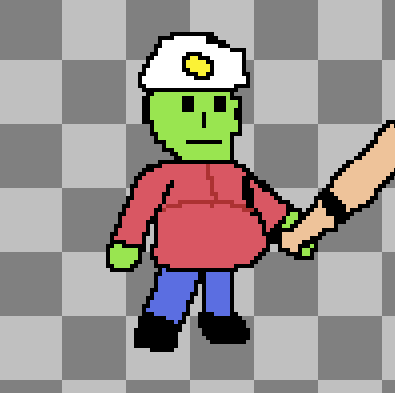
\includegraphics[scale=0.5]{melee.png}
\\
Tank nasprotnik, z melee napadom. Narisal Danijel
\\
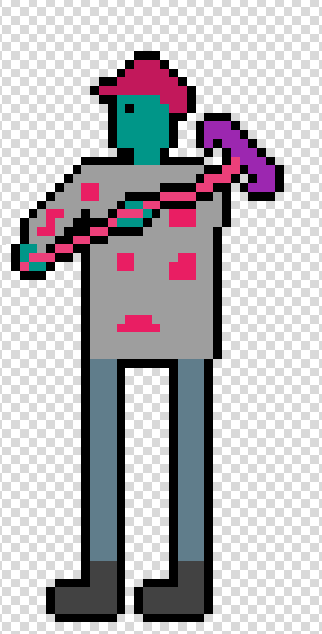
\includegraphics[scale=0.3]{Screenshot_1.png}
\\
Preprosti nasportnik, predstavlja rudarja. Narisal Žan
\\
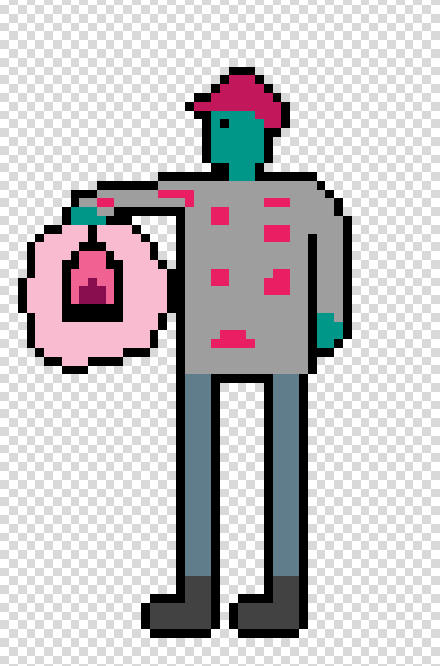
\includegraphics[scale=0.3]{Screenshot_2.png}
\\
Splash damage nasprotnik, predstavlja rudarja, ki te poškoduje z svetlobo od svetilke. Narisal Žan


\end{document}

